%Obviously, the waiting cost of synchronous aggregation is sometime harmful, So we proposed using asynchronous aggregation to reduce the coordination.
%In this section, we first formally define asynchronous aggregation and introduce accumulated recursive aggregation program. We then propose the sufficient conditions for returning correct results by analyzing the aggregate/non-aggregate operations.And then we propose a conversion technology for some unsatisfied algorithm.
%In this section, we propose the foundations of automatic asynchronous aggregation.


\section{Asynchronous Recursive Aggregation}

To support asynchronous processing, we first propose a special form of recursive aggregation, named accumulated recursive aggregation (ARA). Asynchronous execution is only feasible in programs with ARA. We then pose the conditions of that normal recursive aggregation (NRA) can be equally converted to ARA. Finally, we provide the sufficient conditions for correct asynchronous aggregation.

\subsection{Accumulated Recursive Aggregation}
\label{sec:async:accrec}

{
	%\begin{comment}
	\begin{figure*}[t]
		\vspace{-0.1in}
		\centerline{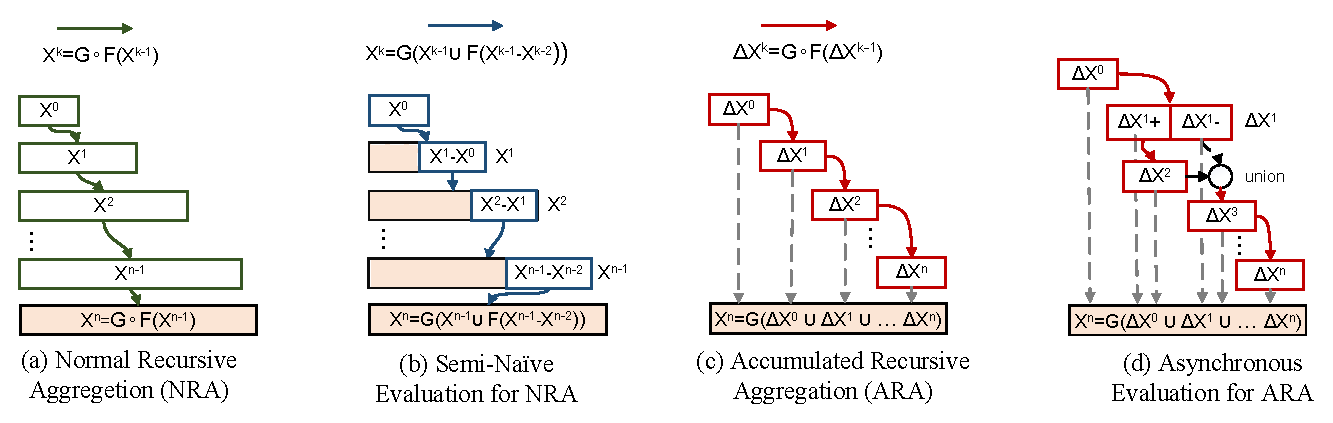
\includegraphics[width=7in]{fig/accumulative.eps}}
		\caption{Normal Recursive Aggregation and Accumulated Recursive Aggregation }
		\vspace{-0.1in}
		\label{fig:arasssp}
	\end{figure*}
	%\end{comment}	
	\textcolor{green}{
		We observed that some of the Recursive aggregation has the potential to be evaluated incrementally, when monotonic conditions are satisfied. i.e., The result of the previous recursion needs to involved in the next recursion. Take SSSP as example, the $\$min$ operation takes both newly generated paths and the current minimum distance as input to find the minimum distance. We find that these program can be rewrite as accumulated recursive aggregation forms that has the potential to asynchronouly processing e.q., Figure \ref{fig:arasssp}. Hence we gives the definition of accumulated recursive aggregation.
	}
	
	\textcolor{red}{
		We observed that some of the Recursive aggregation program has the potential to be asynchronous evaluating when it can be expressed as a special incremental form, i.e., accumulated recursive aggregation. First we give the formal definition.
	}
	
	\begin{definition}
		\label{def:araggre}
		(\textbf{Accumulated Recursive Aggregation.})
		For a normal recursive aggregation as defined with equation \ref{eq:recursive2}, the accumulated recursive aggregation form can be represented as follows.
		\begin{equation}\label{eq:accumasync}
		\begin{aligned}
		\Delta Y^{k}&= F(\Delta X^k)\\
		\Delta X^{k+1}&= G(\Delta Y^{k})\\ 
		X^{n}&=G(\Delta X^0\cup\Delta X^1\ldots\Delta X^{n})
		\end{aligned}
		\end{equation}
		It starts from $\Delta X^0=X^0$ and terminates when there is no new $\Delta Y^k$ produced. The final result is the aggregation of all intermediate results. As shown in Figure \ref{fig:arasssp}.
	\end{definition}
{\color{red}
Evaluating with Equation \ref{eq:accumasync} is not always equivalent with that of Equation \ref{eq:recursive2}. Intuitively, it require the the naive-evaluation of such a program converges to a fixpoint and the result $X$ is monotone. i.e., inducing a partial order $\preceq$  on $X$, $F$ is monotone respect to $\preceq$. we have $X^k\preceq G\circ F(X^{k-1})$, then there exist a finite number $n$ such that

$X^0\succeq G\circ F(X^{0})\ldots \succeq (G\circ F)^n(X^{0})= (G\circ F)^{n+1}(X^{0})$

Then $(G\circ F)^{n}(X^{0})$ is the final result\cite{Lam:2013:SDE:2510649.2511289,Wang:2015:AFR:2824032.2824052}. How ever it is quite hard to determine the sufficient and necessary conditions of monotone.
}
So we proposed a serie of sufficient conditons on converting Normal recursive aggregation to accumulated recursive aggregation which are easy to judge based on the datalog program
	\begin{definition}
		\label{th:monotone}
		(\textbf{Accumulated}) 
		\begin{itemize}
			\item \textbf{commutative}: $G(Y_1\cup Y_2)=G(Y_2\cup Y_1)$
			\item \textbf{monotonic}: $X\subseteq F(X)$
			\item \textbf{accumulative}: $G(Y_1\cup Y_2)=G(G(Y_1)\cup Y_2)$
			%	\item \textbf{idempotent}: $G(Y_1\cup Y_1)=G(Y_1)$
			%\item \textcolor{red}{\textbf{order-independent}}: $G\circ F\circ G(X\cup Y)=G\circ F( G(X)\cup G(Y))$
		\end{itemize}
		A normal recursive aggregate form can be correctly converted to accumulated recursive aggregations, if the aggregate operation $G$ is commutative and accumulative, snd the non-aggregate operations $F$ is monotonic under $G$.
		
		We can easily proof that the accumulated recursive aggregation return the same result with normal recursive aggregation as equation \ref{eq:recursive2} as shown in Appendix \ref{sec:app:proof:monotonic}.
	\end{definition}
	
	{\color{red}
		Accumulative recursive aggregation program has similar form with semi-naive technology. But they are essentially different.
		semi-naive technology is target on reducing redundant computation, The increment of each iteration is computed based on the previous two adjacent step. While accumulated recursive aggregation aims at incrementally evaluating the original datalog program to support asynchronous processing. and the increment is computed iteratively .However, the accumulated recursive aggregation program can also be evaluated with semi-naive technology. if the corresponding conditions are satisfied
	}
	
	
	\subsection{Conditions for Asynchronous Aggregation}
	\label{sec:async:condition}
	\begin{comment}
	\begin{figure}[t]
		\vspace{-0.1in}
		\hspace{-0.3in}
		\centerline{\includegraphics[width=3.6in]{fig/asynchronous.pdf}}
		\caption{Asynchronous and Synchronous Evaluation }
		\vspace{-0.1in}
		\label{fig:asynchronous Evaluation}
	\end{figure}
	\end{comment}
	The recursive program in Definition \ref{def:araggre} is evaluated with synchronous aggregation. 
	In the $k$th iteration, The input of aggregate operation  $\Delta Y^{k-1}$ can be partition into $m$ disjoint part $\{\Delta Y_1^{k-1},\Delta Y_2^{k-1}\ldots \Delta Y_m^{k-1} \}$(value from same key might be divided into two or more subsets).
	
	The synchronous aggregate operation has to wait for all the $m$ subset ready to perform aggregation i.e. $X^k= G( \Delta Y^{k-1})$, before starting the $(k+1)$th round of $F$ operations.  Correspondingly, we define asynchronous aggregation as follows.
	\begin{definition}(\textbf{Asynchronous Aggregation})
		\label{def:asyncaggre}
		Divide the $k$th synchronous non-aggregate output $\Delta Y$ into $m$ arbitrary non-intersect subset $\{\Delta Y_1^{k-1},\Delta Y_2^{k-1}\ldots \Delta Y_m^{k-1} \}$. For the $k$th iteration, the aggregate operation $G$ takes only subset $\Delta Y_{i}^k(1\le i\le m)$ as inputs and the other subset is to be aggregated in later iteration.
	\end{definition}
	
	Given equation \ref{eq:accumasync}, we give an asynchronous evaluating example in Figure \ref{fig:arasssp}. In the $0$th iteration, the nonaggregate output $Y^0$ are divided into two subset $Y^0_+$ and $Y^0_-$, $X^1$ is a partial aggregation based on $Y^0_+$, Then the later iteration is based on 
	And this is also the basic form of asynchronous accumulated recursive aggregation. 
	
	As discussed, asynchronous aggregation is possible in accumulated recursive programs. But not all accumulated recursive programs with asynchronous aggregation will return the same result as that with synchronous aggregation. We demonstrate the sufficient conditions for asynchronous evaluating in the following theorem.
	
	\begin{theorem}
		\label{th:async}
		(\textbf{Asynchronizability}) With asynchronous aggregation as described in Definition \ref{def:asyncaggre}, an accumulated recursive program will yield to the same result as with synchronous aggregation after the $F$ \textcolor{green}{and $G$} operations are performed {\color{green}infinite}the same times with synchronous processing, as long as the following conditions are satisfied.
		\begin{itemize}
			\item \textbf{\textcolor{red}{Accumulable}}: $(G\circ F)^n(X)=G(\Delta X^0\cup\Delta X^1\ldots\Delta X^{n})$;
			\item \textbf{\textcolor{red}{Order-independent}}: $G\circ F\circ G(X)=G\circ F( X)$;
			%	\item \textbf{commutative}: $G(Y_1\cup Y_2)=G(Y_2\cup Y_1)$;
		\end{itemize}
	\end{theorem}
	
	The \textcolor{blue}{order independent} property implies that no matter the $F()$ operation is first applied or the $G()$ operation is first applied, the effect is the same. As long as the same number of $F()$ operations are applied on all the initial inputs and the final operator is $G()$, the eventual aggregation result will be the same.%Due to de definition ,it is obvious that $G$and $F$ operations also satisfied order-independent and commutative properties in this condition.
	We give the formal proof in appendix \ref{},
	
	For the SSSP example, the $F()$ operation expands the BFS searching scope to one-hop-away nodes, and the $G()$ operation picks the minimal distance resulted from the shortest path. The shortest distances are the same no matter making expansion first $G\circ F(X)$ or making aggregation first $F'\circ G(X)$, i.e., for each node $j$, $min_j(d_j+w)=min_j(min_j(d_j)+w)$. There are a broad class of computations that satisfy these conditions and can be executed asynchronously.
	
	%\textcolor{red}{why not using PATH example? I'd like to remove the SSSP example in the paper.}
	\begin{comment}
	For the PATH example, the $F()$ operation broadcast current paths number to all the one-hop-away nodes, and the $G()$ operation sum the paths number from all the in neighbors. The paths number are the same no matter making broadcast $G\circ F(X)$ first or making aggregation first $F\circ G(X)$, i.e., for each node pair $(i,j)$, $sum_{i,j}(p_1,p_2)= sum_{i,j}(sum_{i,j}(p_1),sum_{i,j}(p_2))$. There are a broad class of computations that satisfy these conditions and can be executed asynchronously (Here we give several examples in our technical report \cite{fullversion}).
	
	\end{comment}
	
	
	
